\documentclass[aps,prb,twocolumn,
	groupedaddress,superscriptaddress,
	amsfonts,amssymb,amsmath,floatfix,
	citeautoscript]{revtex4-1}

\usepackage{graphicx}
\usepackage[centering,hmargin=20mm,tmargin=30mm,bmargin=25mm]{geometry}
\usepackage{multirow}
\usepackage{newtxtext}
\usepackage[cmintegrals]{newtxmath}

%----- References -----
\usepackage{xcolor}
\usepackage{hyperref}
\hypersetup{colorlinks,
	linkcolor={blue!75!black!80!yellow},
	citecolor={blue!75!black!80!yellow},
	urlcolor={blue!75!black!80!yellow}
}

%----- Captions in sans font -----
\makeatletter
\renewcommand\@make@capt@title[2]{%
	\@ifx@empty\float@link{\@firstofone}{\expandafter\href\expandafter{\float@link}}%
	\sffamily{\textbf{#1}}\@caption@fignum@sep#2
}%
\renewcommand\figurename{Fig.}
\makeatother

\thickmuskip=5mu plus 2mu minus 1mu  %binary relations (default, 5mu plus 5mu)
\medmuskip=4mu plus 2mu minus 2mu    %binary operations (default, 4mu plus 2mu minus 4mu)

\frenchspacing %Ensure that revTeX does not do "double spaces" after punctuation

\renewcommand{\Im}{\operatorname{Im}}
\renewcommand{\Re}{\operatorname{Re}}
\newcommand{\sub}[1]{\ensuremath{_{\textrm{#1}}}} %Upright multi-character subscript
\newcommand{\super}[1]{\ensuremath{^{\textrm{#1}}}} %Upright multi-character superscript

\newcommand{\HarvardSEAS}{John A. Paulson School of Engineering and Applied Sciences, Harvard University, Cambridge, MA, USA}
\newcommand{\MITPhy}{Department of Physics, Massachusetts Institute of Technology, Cambridge, MA, USA}

\usepackage[normalem]{ulem}
\newcommand{\Jadd}[1]{\textcolor{blue}{#1}}
\newcommand{\Jrem}[1]{\textcolor{blue}{\sout{#1}}}


%\usepackage[usenames]{color}
%\newcommand{\edited}[1]{{\color{red} #1}}

\begin{document}

\title{Variational theory of the ground state of quantum electrodynamics}

\author{Nicholas Rivera}\email{nrivera@seas.harvard.edu}\affiliation{\HarvardSEAS}\affiliation{\MITPhy}
\author{Johannes Flick}\email{flick@seas.harvard.edu}\affiliation{\HarvardSEAS}
\author{Prineha Narang}\email{prineha@seas.harvard.edu}\affiliation{\HarvardSEAS}


\date{\today}

\begin{abstract}
The past decade has brought rapid theoretical and experimental advances in the field of ultra-strong coupling of light and matter from microwave to optical frequencies. Many of the theoretical analyses of such systems proceed by considering simple two-level systems coupled to a single cavity mode. There remains a need to understand light-matter coupling  in contexts of complicated electronic systems coupling to many-mode or continuum photonic systems. A promising recent development along these lines is quantum electrodynamical density functional theory, which describes the ground state of a QED system in terms of reduced quantities such as the electronic density and electromagnetic displacement field. 
In this work, we complement the set of theoretical tools for describing ground states of light-matter systems by developing a variational theory of the ground state of a quantum electrodynamical system of coupled light and matter. Essential to our ansatz is the notion an effective photonic vacuum whose modes are different than the modes in the absence of light-matter coupling. As a first step towards an eventually \textit{ab initio} approach to ground states in QED, we apply our ansatz to a Rabi model involving a multi-level emitter with many optical modes, a model which cannot be analytically solved. We find a compact semi-analytic formula which describes the ground state energy very accurately (to less than 1\% error) in all regimes of coupling parameters allowed by the Thomas-Reiche-Kuhn sum rule. 
\end{abstract}

\maketitle

\section{Introduction}
\label{sec:Introduction}

The past decade has brought an explosion of effort and experimental progress in realizing the coupling of matter and quantized electromagnetic fields beyond a regime of weak coupling, in which perturbative treatments of quantum electrodynamical couplings can no longer accurately describe the dynamics \cite{flick7strong,ruggenthaler2017b,forn2018ultrastrong,kockum2018ultrastrong}. Ultra-strong, or even deep-strong coupling is now regularly observed in superconducting qubits at microwave frequencies \cite{blais2004,wallraff2004,yoshihara2017superconducting,forn2017ultrastrong}, ensembles of molecules in optical cavities \cite{hutchison2012,hutchison2013,coles2014,coles2014b,shalabney2015coherent, thomas2016,ebbesen2016}, 2D electron gas cyclotron resonances coupled to cavities \cite{hagenmuller2010ultrastrong,scalari2012ultrastrong,zhang2016collective}, intersubband transitions in quantum wells coupled to cavities \cite{todorov2010ultrastrong,geiser2012ultrastrong}, and single-emitters in ultra-confined plasmonic geometries \cite{benz2016,chikkaraddy2016}. Proposals for new platforms of ultra-strong coupling include emitters coupling to highly confined polaritons in metals and polar insulators \cite{rivera2016shrinking}, highly ionized atoms coupled to optical media via the Cerenkov effect, and many more. The proposed applications for ultra- and deep-strong coupling of light and matter are similarly broad, including simulation of many-body systems \cite{forn2018ultrastrong}, altering chemical reactivity~\cite{hutchison2012, thomas2016,flick2017} and electronic transport properties \cite{orgiu2015}, realizing analogues of nonlinear optical processes with vacuum fluctuations \cite{kockum2017deterministic}, and even as new sources of photons through the dynamical Casimir effect \cite{ciuti2005quantum}.

In the nonperturbative regime of quantum electrodynamics, there are very few models which can be analytically solved. In particularly, the only exactly solvable models in all regimes of coupling parameters include the Rabi model~\cite{braak2011}, which describes the coupling of a two-level atom to a single mode, the Hopfield model \cite{hopfield1958theory}, which describes the coupling of a harmonic oscillator to any number of cavity modes, and Dicke models based on two-level systems and harmonic oscillators \cite{dicke1954coherence}. Any realistic system which deviates from these simpler models require numerical diagonalization approaches, which become unwieldy when the dimension of the electronic Hilbert space becomes large, as is the case when describing an electronic system in real space. It also becomes unwieldy when one needs to keep track of many cavity modes, which can be populated with many photons. Exciting new developments towards ab-initio studies of QED have proceeded by proposing reduced-quantity descriptions such as density-functional descriptions of the light-matter coupling \cite{ruggenthaler2014,pellegrini2015,flick2015,dimitrov2017,flick2018,flick2018b,schaefer2018}. With such density-functional descriptions, workers in this field have been able to compute ground-state and time-dependent properties of realistic molecules in optical cavities \cite{flick2017c}. 

In what follows, we propose the use variational methods for the solution of \emph{ab initio} QED problems. In particular, here we develop a particular class of mean-field variational ansatzes for the ground state of quantum electrodynamical Hamiltonians. In particular, we develop an ansatz in which the ground state can be considered as a factorizable state of an effective matter and effective photon quasiparticle both in their respective ground states. This ansatz, analogous to the Hartree-Fock ansatz of electronic structure theory, leads to coupled eigen-equations describing the ground-state of the light-matter system. We benchmark our ansatz against a multi-level and multi-mode Rabi model parameterized by the strength of the characteristic momentum matrix elements describing the coupling of the matter and the electromagnetic fields. We find that when the momentum matrix elements are sufficiently weak, our theory finds the ground state energy to a remarkable accuracy of less than >99.9\%, even in the non-perturbative coupling regime. Even in regimes where the correlation energy is 50\% of the total energy, far outside of the validity domain of our ansatz, our ansatz predicts the energy up to a few percent. In regimes where our results are accurate, we claim we have found the effective quasiparticle description of the ground state. Moreover, in this regime, the ground state interaction energy manifests itself as the difference in zero-point energies between the quasiparticles and the bare particles. This generalizes the notion of the Casimir energy to a single atom in a cavity.

Our results service several aims. First, they suggest a novel variational approach for understanding ground states in ultra-strongly coupled light-matter systems. Second, they provide a general framework for understanding light-matter decoupling effects in the regime of strong light-matter interactions. Third, they prove a non-perturbative theory of Casimir-Polder forces. Finally, they provide a rigorous concept of correlation energy in quantum electrodynamics in a way analogous to electronic structure theory. 

The outline of this work is as follows: in section~\ref{sec:variational_ansatz}, we develop the variational ansatz for the ground state of the Hamiltonian of macroscopic quantum electrodynamics. In section~\ref{sec:multi-level}, we calculate the ground state energy according to this ansatz for the multi-level and multi-mode Rabi model and compare it to numerical diagonalization of the same problem. In Section~\ref{sec:extensions}, we propose a self-consistent extension of our ansatz. 

\section{Theory}
\label{sec:theory}
In the Supplementary Information (SI), we derive a set of nonlinear coupled eigenequations which can be applied to describe the ground state of any macroscopic quantum electrodynamical system, in three dimensions, with electron-electron interactions, and with arbitrarily many photon modes. These are real-space equations that give single-particle electron and photon orbitals in the presence of QED coupling, thus giving real-space information about the electron density and the electromagnetic field fluctuations in the ground state. The equations derived are in general fairly complicated, and thus in the main text, we analyze a much simpler case of the equations in order to extract the basic physics of the equations. 

In the main text, we consider the light-matter Hamiltonian corresponding to a single emitter placed at position $z=d$ in a one-dimensional cavity oriented along the $z$-direction. As the cavity is considered for simplicity to be one-dimensional, the electric field is oriented along a single direction, denoted $x$, while the magnetic field is oriented along a direction transverse to both the electric field and the cavity length, denoted $y$. We consider the interaction in the velocity gauge, and neglect the weak interaction between spins and magnetic fields, thus neglecting spin altogether. The Hamiltonian can then be written as:
\begin{equation}\label{eq:hamiltonian}
H = H_{\text{matter}}+\frac{\epsilon_0}{2}\int dz~(E^2+c^2B^2)+\frac{q}{m}A(d)p + \frac{q^2}{2m}A^2(d).
\end{equation}
The fields can be expressed as a mode expansion via:
\begin{equation}\label{eq:mode_expansion}
A(z,t) = \sum\limits_{n=1}^{\infty} \sqrt{\frac{\hbar}{2\epsilon_0\omega_n }}(F_n(z)a_ne^{-i\omega_n t}+F^*_n(z)a_n^{\dagger}e^{i\omega_n t}),
\end{equation}
with $E(z,t) = -\partial_t A(z,t)$ and $B(z,t)=\partial_z A(z,t)$.  The $F_n(z)$ are the mode functions of the cavity, normalized such that $\int dz ~|F_n(z)|^2 = 1$. For a cavity of length $L$ the modes are given by $F_n(z) = \sqrt{\frac{2}{L}}\sin\left(\frac{n\pi z}{L} \right)$ and the corresponding mode frequencies are $\omega_n = \frac{n\pi c}{L}$. The matter Hamiltonian we take to be a multilevel system with an arbitrary number of levels, $N_a$. The matter system we describe as an $N_a$ site system. This could be considered as a simple model of a molecule within a tight-binding description. Thus we parameterize the general family of matter Hamiltonians as:
\begin{equation}\label{eq:matter_hamiltonian}
H_{\text{matter}} = \sum\limits_{i=1}^{{N_a-1}} V_i|i\rangle\langle i|+t(|i\rangle\langle i+1|+|i+1\rangle\langle i|) 
\end{equation}
The momentum operator, we write in a finite-different representation as
\begin{equation}\label{eq:momentum_operator}
p = \frac{-i\hbar}{R}\sum\limits_{i=1}^{N_a-1} \left(|i\rangle\langle i+1|-|i+1\rangle\langle i| \right),
\end{equation}
where $R$ is a constant with units of length representing roughly the difference in positions between sites. This physical interpretation however is rough: it is also a function of the hopping elements $t$, because we choose $R$ in this work such that the following sum rule is enforced: 
\begin{equation}\label{eq:TRK_sum_rule}
\frac{2}{m}\sum\limits_{i=2}^{N_a}\frac{|p_{ig}|^2}{E_i - E_a} = 1,
\end{equation}
where $p_{ig} = \langle i|p|g\rangle$ are momentum matrix elements between different matter states. Equation \ref{eq:TRK_sum_rule} is the Thomas-Reiche-Kuhn (TRK) sum rule. Of course, this sum rule does not rigorously apply to a discrete-level system. However, the matrix elements and energy levels of a few-level approximated Hamiltonian  are derived from an underlying real-space (infinite dimensional) Hamiltonian, a discrete system which has  $\frac{2}{m}\sum\limits_{i=2}^{N_a}\frac{|p_{ig}|^2}{E_i - E_a} > 1$ cannot. As we shall show later in the text however, it does place a bound on how strong the effect of the $Ap$ term can be on the total energy. The net effect is that the value of $R$ we choose is on the order of $\sqrt{\frac{\hbar}{2mt}}$.

\section{Variational ansatz}
\label{sec:variational_ansatz}
\begin{figure*}[t]
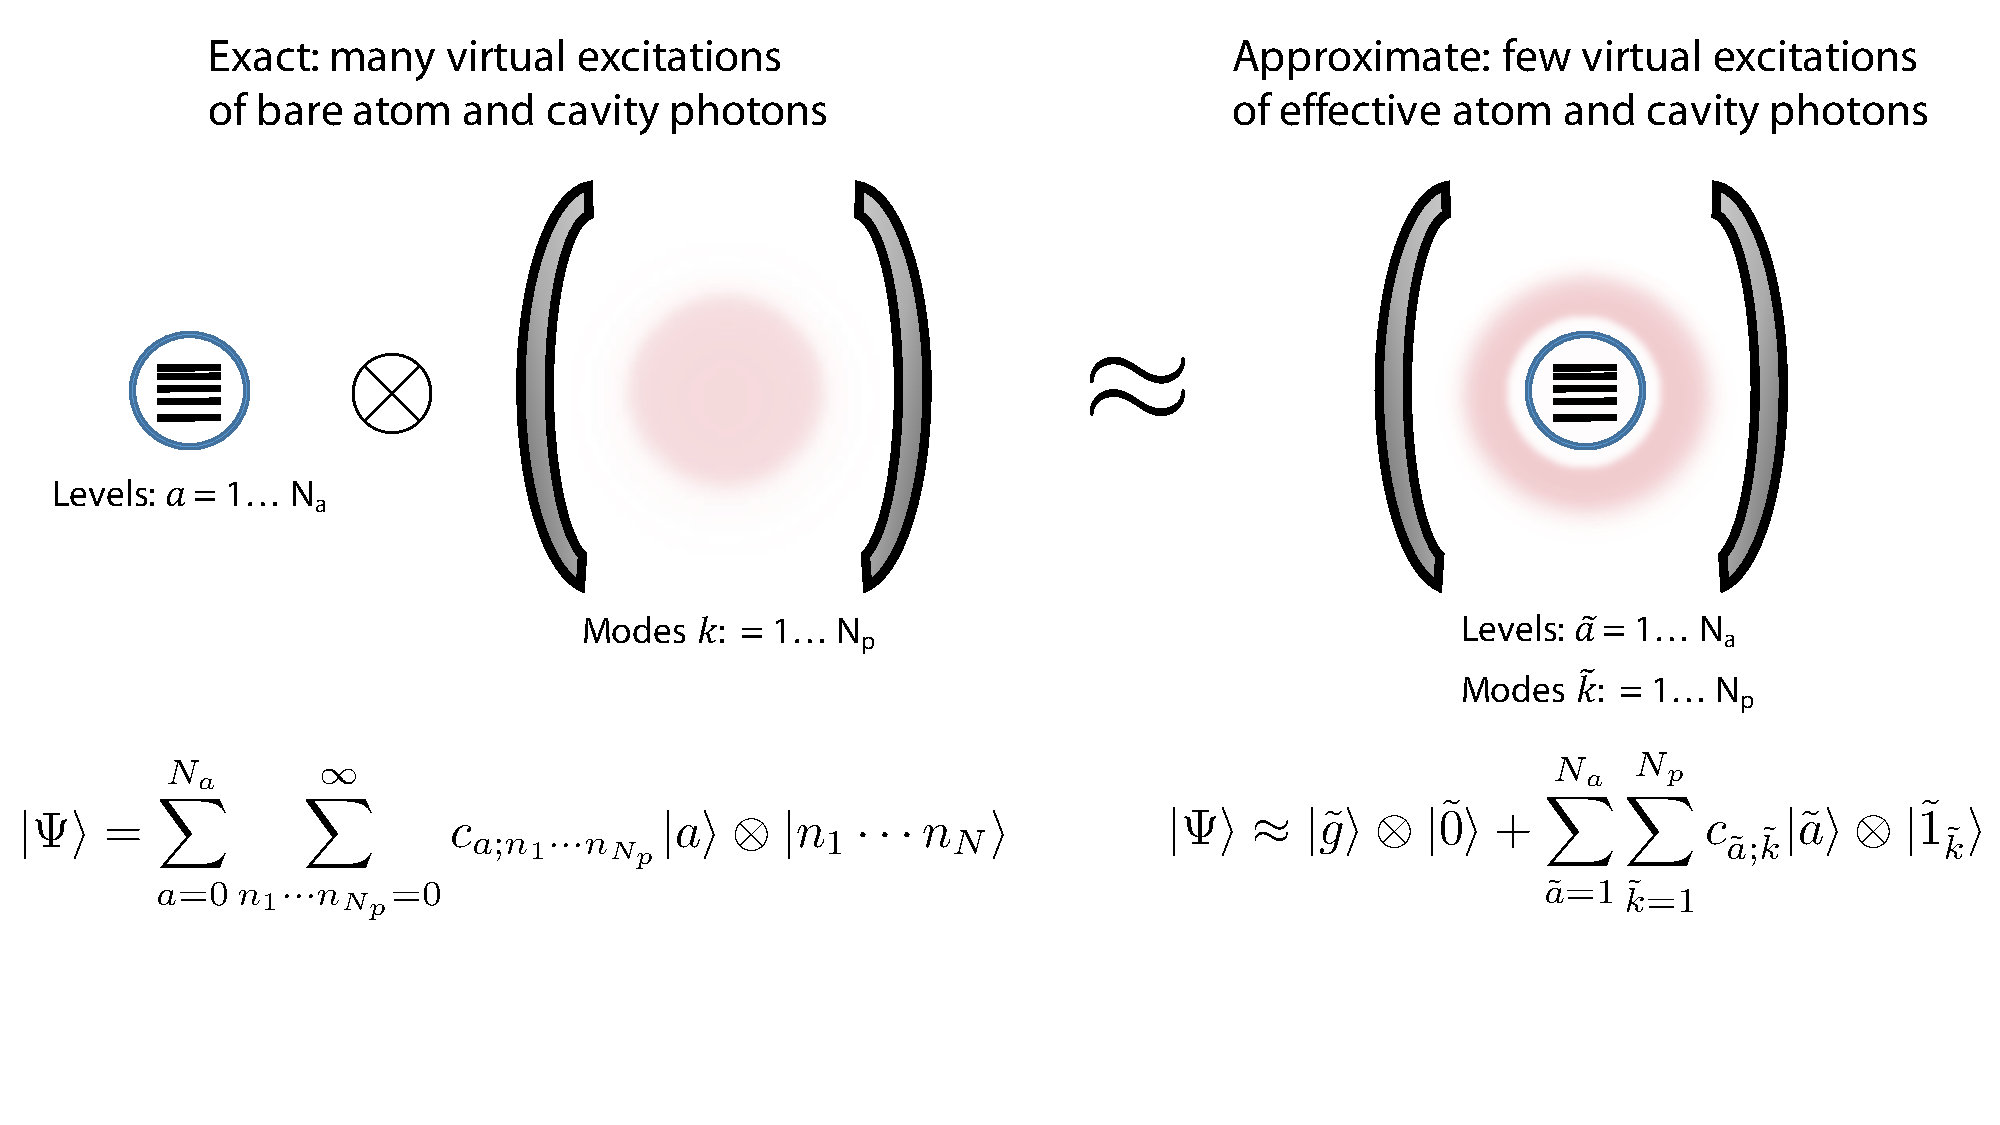
\includegraphics[width=16cm]{conceptfigure.pdf}
\caption{\textbf{Ground-state ansatz applied to matter in a cavity: effectively decoupled matter and photons.} (Left) Bare description of the coupled light-matter ground state in terms of many virtual excitations of the emitter state and the bare cavity photons. (Right) Quasiparticle description of the coupled system as a factorable state an effective emitter in its ground state and the vacuum of an effective photonic degree of freedom.}
\label{fig:ansatz}
\end{figure*}

The concept behind the variational ansatz is shown in Figure~(\ref{fig:ansatz}). We seek a description of the ground state of the system as $|\Psi\rangle \approx |\tilde{g}\rangle\otimes|\tilde{0}\rangle + |\delta\rangle,$ where a $\sim$ denotes an effective quantity. In other words, we seek a description in which the state is a factorizable state of matter and photon \textit{quasi}particles, up to some correlations quantified by the state $|\delta\rangle$. These correlations essentially hybridize $|\tilde{g}\rangle\otimes|\tilde{0}\rangle$ with excitations of the effective emitter and virtual effective photons. 

We start our analysis by considering a family of ansatze in which $\delta = 0$ (uncorrelated ansatz).  The expectation value of the Hamiltonian is %\Jadd{(the matter part is assumed to be a single atom, we could use the density here.)}
\begin{align}\label{eq:expectation_val1}
\langle \Psi | H | \Psi \rangle &= \langle \tilde{g} |H_{\text{matter}} | \tilde{g}\rangle \nonumber \\ &+ \frac{\hbar}{4}\int dz ~\sum\limits_{n=1}^{\infty}\left(\omega_n|F_n|^2 - \frac{c^2}{\omega_n}F_n^*\partial_z^2F_n\right) \nonumber \\ &+ \frac{\hbar q^2}{4m\epsilon_0\omega_n}\sum\limits_{n=1}^{\infty} \int dz~\delta(z-d)|F_n|^2
\end{align}
Notably, in this ansatz, the term in the Hamiltonian coupling the momentum of the matter to the photon makes no contribution. We impose constraints of matter normalization and photon mode normalization by defining a Lagrange function 
\begin{align}\label{eq:lagrange}
&\mathcal{L}(\Psi, \Psi^*, \{F_n, F_n^*, \omega_n, \lambda_n\}) \equiv \langle \Psi | H | \Psi \rangle \nonumber \\ &- \epsilon(\langle \tilde{g}|\tilde{g}\rangle-1)-\sum\limits_{n=1}^{\infty}\frac{\hbar\lambda_n}{2}\left( \int dz~|F_n|^2-1\right).
\end{align} 
To find the ground state, we minimize the Lagrange function with respect to the matter orbital $|\tilde{g}\rangle$ and with respect to the mode functions $F_n$. The minimization with respect to the matter leads to the trivial equation $H_{\text{matter}} |\tilde{g}\rangle = \epsilon|\tilde{g}\rangle$ which leaves the effective matter ground state as simply the ground state of $H_{\text{matter}}$. On the other hand, the minimization with respect to the photon mode functions leads to  the equation
\begin{equation}\label{eq:maxwell}
\left(\partial_z^2-\frac{\omega^2_n}{c^2}+2\frac{\omega_n\lambda_n}{c^2}-\frac{q^2 }{m\epsilon_0 c^2}\delta(z-d)\right)F_n  = 0.
\end{equation}
We may constrain the $\lambda_n$ by differentiating the Lagrange function also with respect to the $\omega_n$. The equation which follows is:
\begin{equation}\label{eq:other_maxwell}
\int dz ~\left(|F_n|^2 + \frac{c^2}{\omega^2_n}F_n^*\partial_z^2F_n\right) - \frac{ q^2}{m\epsilon_0\omega^2_n} \int dz~\delta(z-d)|F_n|^2 = 0
\end{equation}
Performing $\frac{\omega_n^2}{c^2}\int dz~F_n^*$ on both sides of Equation \ref{eq:maxwell}, and adding this equation to Equation \ref{eq:other_maxwell}, one immediately finds that $\lambda_n = \omega_n$ and that
\begin{equation}\label{eq:final_maxwell}
\left(\partial_z^2+\frac{\omega^2_n}{c^2}-\frac{q^2 }{m\epsilon_0 c^2}\delta(z-d)\right)F_n  = 0.
\end{equation}
\begin{figure*}[t]
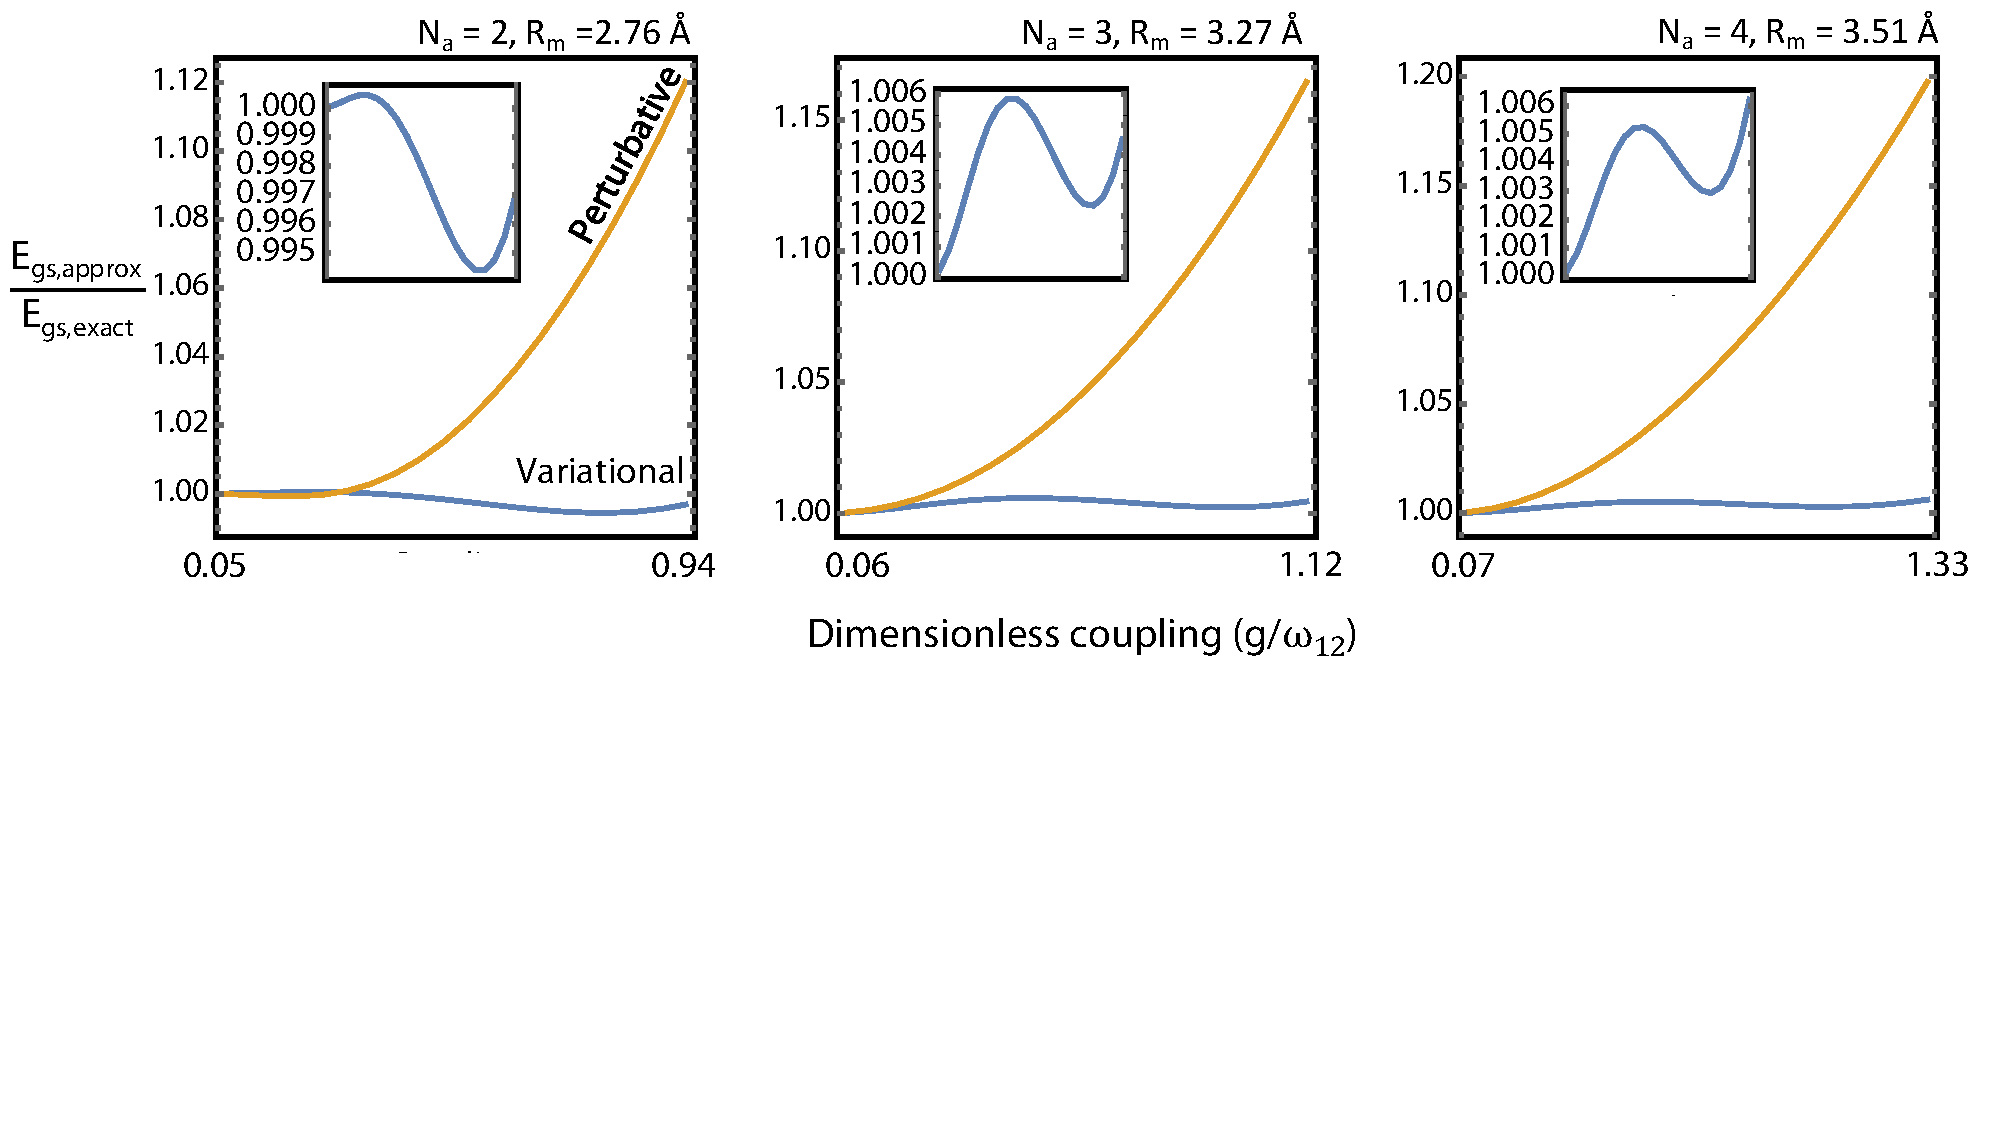
\includegraphics[width=16cm]{fig2.pdf}
\caption{\textbf{Comparison of the accuracy of the variational ansatz to exact diagonalization of the multi-level and multi-mode Rabi model.} Ratio of approximate ground state energy (calculated via our ansatz and perturbatively) to the energy obtained by numerical diagonalization of the Hamiltonian, truncating the Hilbert space to four photons for (left) a two-level system, (middle) a three-level system, and (right) a four-level system. The length parameter which sets the strength of the momentum matrix elements is chosen to saturate the TRK sum rule.}
\label{fig:decoupling}
\end{figure*}
This is an ordinary second-order differential equation with the conditions that $F_n$ is continuous at $d$ and that its derivative is discontinuous according to 
\begin{equation}\label{eq:boundary_condition}
\partial_zF_n\Big|_{z=d^+}-\partial_zF_n\Big|_{z=d^-} = \frac{q^2}{m\epsilon_0 c^2}F_n(d),
\end{equation}
in addition to the usual condition of the modes vanishing at the cavity walls $z=0$ and $z=L$. It can be shown that the solution to Equation \ref{eq:final_maxwell} satisfying such boundary conditions is:
\begin{align}\label{eq:field_mode}
&\theta (z-d) \left(\frac{\sin\left(\frac{\omega_nL}{c}\right)\sin\left(\frac{\omega_nd}{c}\right)\cos\left(\frac{\omega_nz}{c}\right)}{\sin\left(\frac{\omega_n(L-d)}{c}\right)}-\right) \nonumber \\ 
-&\theta (z-d) \left(\frac{\cos\left(\frac{\omega_nL}{c}\right)\sin\left(\frac{\omega_nd}{c}\right)\sin\left(\frac{\omega_nz}{c}\right)}{\sin\left(\frac{\omega_n(L-d)}{c}\right)}\right) \nonumber \\ 
+&\theta (d-z) \sin\left(\frac{\omega_n z}{c} \right)
\end{align}
provided that the auxiliary condition
\begin{equation}\label{eq:mode_transcendental}
\cot\left(\frac{\omega_n}{c}d \right)+\cot\left(\frac{\omega_n}{c}(L-d) \right) = \frac{q^2}{4m\epsilon_0\omega_nc}
\end{equation}
is met. To ensure that the modes are normalized according to the constraint, we have that the solutions of Equation \ref{eq:field_mode} must be multiplied by a normalization factor $N_n$ given by
\begin{equation}\label{eq:mode_normalization}
N_n = 2\sqrt{\frac{c}{\omega_n\left(\frac{\omega_nL}{c}-\sin\left(\frac{\omega_nL}{c}\right) \right)\left(1+\frac{\sin^2\left(\frac{\omega_nd}{c}\right)}{\sin^2\left(\frac{\omega_n(L-d)}{c}\right)} \right)}}.
\end{equation}
The condition of Equation \ref{eq:mode_transcendental} determines the resonance frequencies of the photon quasiparticle modes. After calculating the modes and the frequencies, we may move to an evaluation of the energy of the ground state. We proceed by taking the solutions of Equation \ref{eq:field_mode}, normalized with the normalization factor of Equation \ref{eq:mode_normalization}, and plugging it back into the expectation value of the Hamiltonian of the ground state (Equation \ref{eq:expectation_val1}). We find that
\begin{equation}\label{eq:casimir}
\langle \Psi | H|\Psi\rangle = E_{g}+\frac{1}{2}\sum\limits_{n=1}^{\infty}\hbar\omega_n.
\end{equation}
The interaction energy, which is the difference between the ground state energy with $q\neq 0$ and the non-interacting ground state energy, is $\frac{1}{2}\sum\limits_{n=1}^{\infty}\hbar(\omega_n-\omega_n^0)$, where $\omega_n^0 = \frac{n\pi c}{L}$ are the frequencies of the bare cavity modes. The result just derived establishes that the interaction energy within this ansatz is the Casimir energy of the system. This is quite interesting as typically when one calculates a Casimir energy, what is calculated is the zero-point energy associated with the electromagnetic modes of \textit{macroscopic polarizable objects}. Here on the other hand, we consider the \textit{electromagnetic modes of a single atom in a cavity}.

We now look to understand the effect of correlations on our ansatz. Interestingly, at lowest-order, correlations are entirely a result of the coupling between the momentum and the vector potential. Here, we capture the effect of correlations perturbatively. We briefly note that in the context of quantum chemistry, the perturbative approach we take now is analogous to Moller-Plesset perturbation theory (MP2). Treating such correlations perturbatively, it follows that the change in the ground state wavefunction $|\delta\rangle$ is given to first order as:
\begin{equation}\label{eq:MP2wavefunction}
|\delta\rangle = \sum\limits_{b = 2}^{N_a}\sum\limits_{n=1}^{\infty} \frac{q}{m}\sqrt{\frac{1}{2\epsilon_0\omega_n}}\frac{F_n(d)p_{ba}}{\omega_{ab}-\omega_n}|b\rangle|n\rangle.
\end{equation}
The corresponding change in the ground state energy, defined as the correlation energy $E_c$, is
\begin{equation}\label{eq:MP2energy}
E_{c} = \frac{q^2}{2m^2\epsilon_0\omega_n}\frac{|F_n(d)p_{ba}|^2}{\omega_{ab}-\omega_n}.
\end{equation}
Summarizing the result of this section, the quantum electrodynamics interaction energy in the ground state, according to our variational ansatz, should be well-approximated by
\begin{equation}\label{eq:total_interaction_energy}
E_{int} = \frac{1}{2}\sum\limits_{n=1}^{\infty}\left(\hbar\omega_n - \hbar\omega_n^{(0)} \right) + \frac{q^2}{2m^2\epsilon_0\omega_n}\frac{|F_n(d)p_{ba}|^2}{\omega_{ab}-\omega_n},
\end{equation}
where the eigenmodes $F_n$ and their eigenfrequencies $\omega_n$ are given by Equations (12-14).

\section{Application to a multi-level system coupled to a multi-mode cavity}
\label{sec:multi-level}

In this section, we test the validity of the ansatz proposed and developed in the previous section. In particular, we consider an atomic system of varying number of levels (two through four), and a cavity with fifty modes: this system cannot be solved analytically. In particular, the Rabi model can only be solved analytically for a two level system interacting with one cavity mode. 

In Figure~\ref{fig:decoupling}, we consider the ground state energy of the Hamiltonian of Equation \ref{eq:hamiltonian}  calculated by Equation \ref{eq:total_interaction_energy} and also calculated by perturbation theory. By "calculated by perturbation theory", we mean that we apply perturbation theory in which the photonic modes used are the bare sine modes, rather than those of Equation \ref{eq:field_mode}.  In Figure~(\ref{fig:decoupling}) we take the ratio of these ground state energies to the "exact" ground state energy, computed by numerical diagonalization of the Hamiltonian. To do so, we must truncate the Fock space for the photons. For the range of couplings considered in Figure~\ref{fig:decoupling}, up to four photons are needed in the Hilbert space, rendering the dimension of the Hilbert space in the problem to be $6.25\times10^6 \times N_a$ with $N_a$ the number of atomic levels. For two, three, and four-level systems, we find that our ansatz captures the ground state energy derived by numerical diagonalization nearly exactly, within an error of less than 1\%. On the other hand, perturbation theory can feature an error of over 20\% for the largest coupling considered on this plot. The level of accuracy appears to be independent of the number of levels, suggesting that our accuracy is not an artifact of a two-level approximation. It is also important that our ansatz does well in a multi-level system, because as pointed out recently, there are severe discrepancies between the Coulomb gauge and length gauges for few level systems~\cite{schaefer2018, bernardis2018}, and the slow decay of matrix elements as a function of energy suggests that for few level systems, the length gauge is the appropriate gauge.

Before moving to further analyze the results, we note that we vary the coupling by varying the charge $q$. In principle, we could vary the coupling by varying the strength of the momentum matrix elements, which are controlled by $R$. However, there is a minimum $R=R_{m}$ that is allowed by the TRK sum rule. When $R < R_m$, there is no real-space matter system that our TRK-violating  few-level model can be an approximation of. Thus, in all cases, we chose $R=R_m$ as the value, thus taking the effect of correlations to be as large as they can possibly be.

\begin{figure}[t]
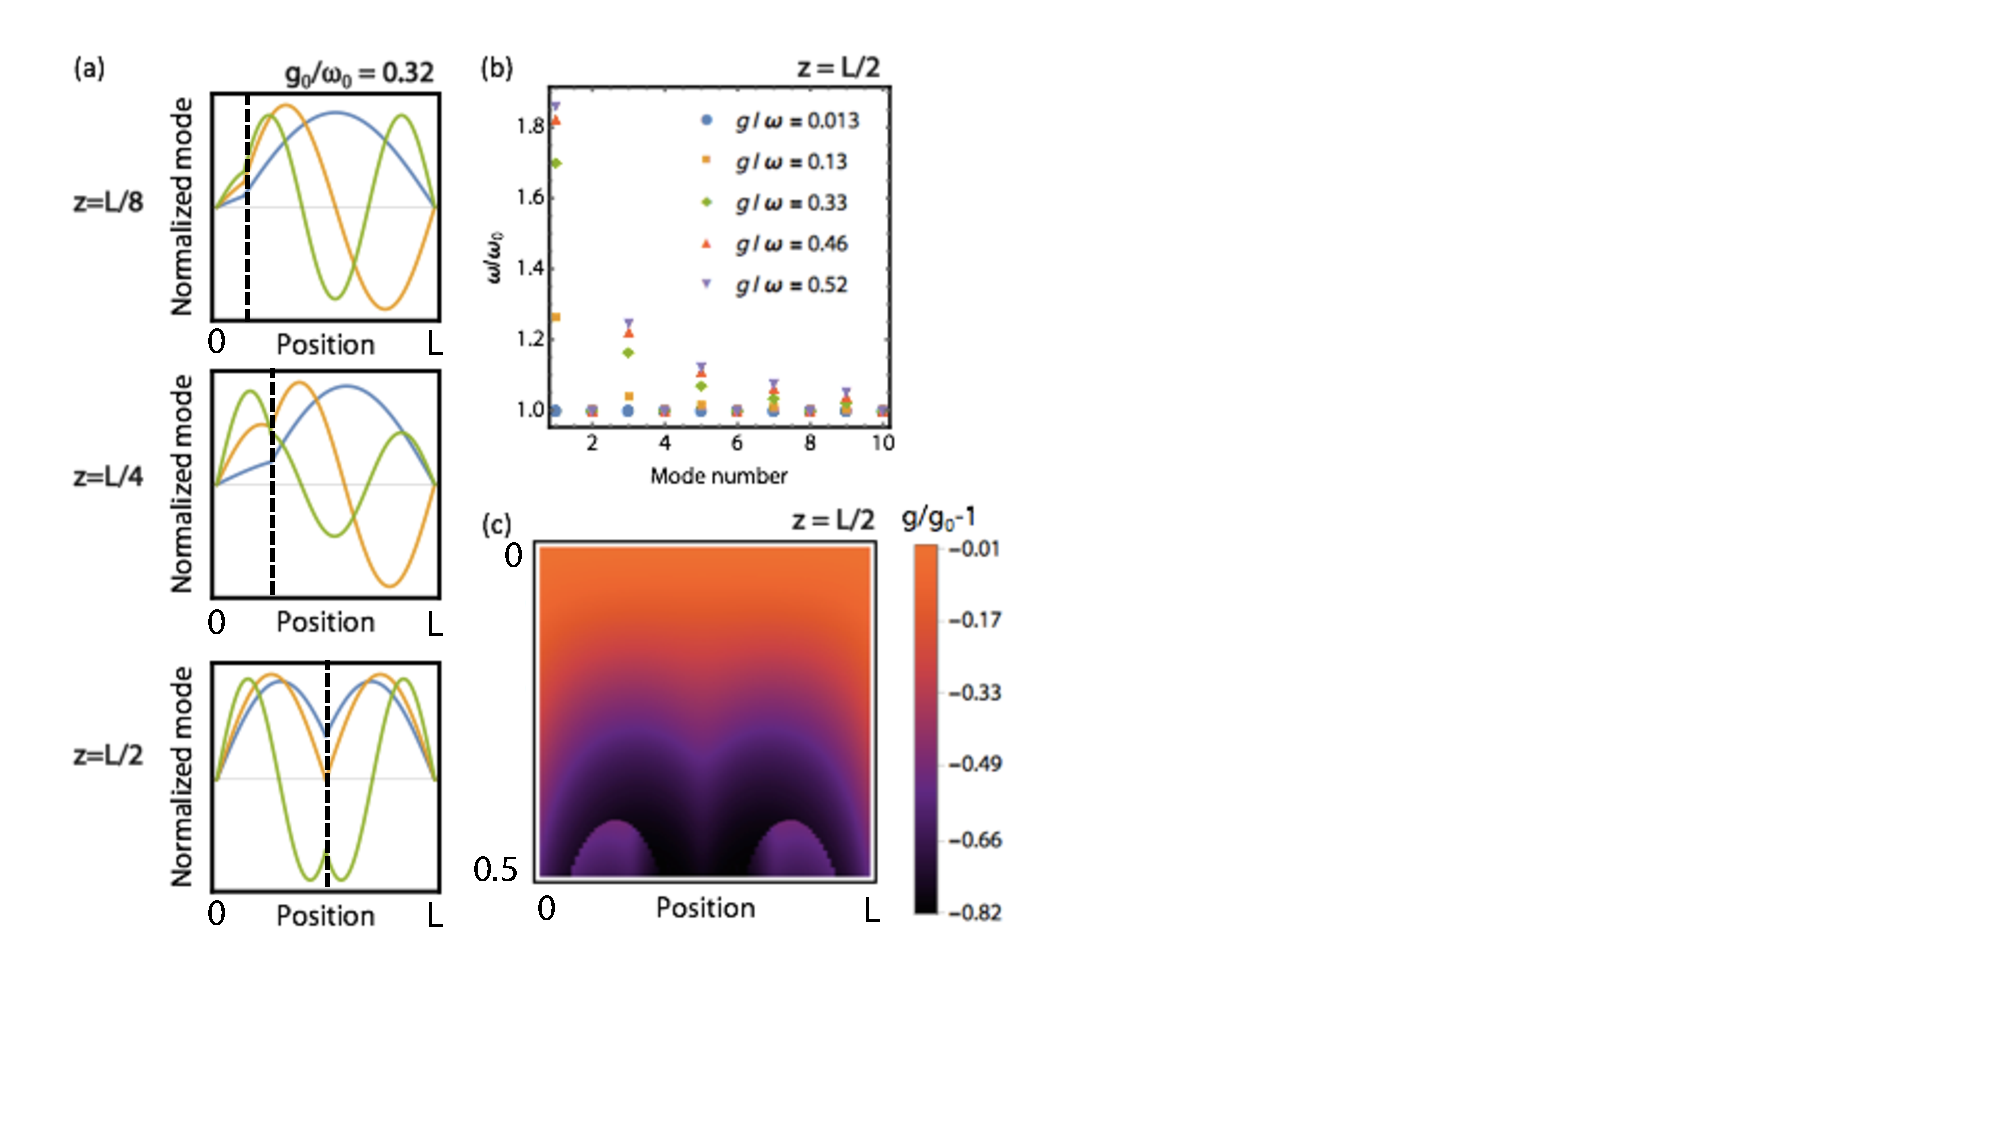
\includegraphics[width=9cm]{fig3.pdf}
\caption{\textbf{Sources of light-matter decoupling in the QED ground state.} (a) Plots of the mode profile of Equations (12-14) for the lowest mode as a function of position in the cavity for different emitter positions. The most striking effect is the screening of the cavity fields in the emitter region, which is most pronounced when the emitter is in the middle of the cavity and interacts strongest with the bare cavity mode. (b) Frequencies of the first ten modes as a function of coupling when the emitter is placed in the center of the cavity. (c) Normalized change in the coupling constant between matter and electromagnetic fields as a function of position in the cavity and coupling constant, assuming that the emitter is placed in the center of the cavity.  }
\label{fig:sources_decoupling}
\end{figure}

In Figure~\ref{fig:sources_decoupling}, we explore an interesting feature of Figure ~\ref{fig:decoupling}, which is that the ground-state energy predicted by our ansatz is always substantially lower than predicted by perturbation theory for the coupling parameters considered here. To elaborate on this, we refer to Figure ~\ref{fig:sources_decoupling}(a), which shows the normalized lowest frequency electromagnetic mode $F_1(z)$ given by Equations (12-14) for a coupling strength of $0.33\omega_{21}$ and for different positions of the emitter in the cavity. The most obvious feature one sees is a strong dip (screening) in the electromagnetic fields where the emitter is. An analogous effect, known as a light-matter decoupling effect~\cite{liberato2014,garcia2015light,bayer2017terahertz}, was noted in a recent work analytically in the context of expectation values of photodetection signals in the Hopfield model in cavity QED in the limit of deep-strong coupling. This dip can be understood physically as a result of the fact that the $A^2$ term in the Hamiltonian is positive-definite, increasing the energy when the emitter overlaps with strong intensity of the vacuum fluctuations of the electromagnetic field. Thus the ground state should screen the electromagnetic field fluctuations out of the region where the emitter is. This dip leads to a self-consistent decrease in the magnitude of the interaction energy between the matter and the electromagnetic field, both for the $A^2$ and $Ap$ terms. 

Another feature in Figure~\ref{fig:sources_decoupling}(b) which also leads to a decrease in the magnitude of the interaction relative to perturbation theory is a blue shift of all of the modes relative to their unperturbed values. This is consistent with the fields being pushed out of the emitter region, which increases the curvature of the mode functions. The effect of this blue-shift to reduce the coupling can be seen from the form of the vector potential of a single photon in mode $n$, which depends on the mode via $\frac{F_n}{\sqrt{\omega_n}}$. Thus a blue-shift in the frequencies self-consistently decreases the magnitude of the coupling constant. Additionally, blue shifts lead to a further detuning in the energy denominators of Equations \ref{eq:MP2wavefunction} and \ref{eq:MP2energy}, serving to also self-consistently reduce the effect of correlations. The combined effects of the field screening and blue shifts are summarized in Figure ~\ref{fig:sources_decoupling}(c), where we plot the normalized change in the self-consistent coupling constant 
\begin{equation}
\frac{g_n-g_n^{(0)}}{g_n^{(0)}} = \frac{q}{mR}\sqrt{\frac{\hbar}{2\epsilon_0}}\left(\frac{F_n(d)}{F^{(0)}_n(d)}\sqrt{\frac{\omega^{(0)}_n}{\omega_n}}-1\right)
\end{equation}
for $n=1$ and $b=2$. As can be seen, for bare coupling constants approaching $0.5$, well into the ultra-strong coupling regime, the self-consistent coupling can be reduced by over 80\% as a result of the field screening and blue-shifts.

%\Jadd{(Nick, do you solve it actually in a scf cycle? if so, we could also show how the energy converges per iteration)}

\section{Extensions}
\label{sec:extensions}
Moving forward, there are a few interesting ways to proceed with this ansatz. Of course, in the spirit of recent work on ab-initio treatments of quantum electrodynamics, it will be of great interest to apply this ansatz on problems involving realistic molecules ultra strongly coupled to cavities, and other photonic and plasmonic platforms which facilitate the ultra-strong coupling of light and matter. To do this, one must take into account the effect of electronic interactions. Another interesting direction is to apply this ansatz on a system in which a perturbative treatment of correlations fails to capture their effect accurately. One way to remedy this in the framework of our ansatz is to treat the terms in the correlation energy of Equation \ref{eq:MP2energy} as variational parameters: this leads to a revised set of equations for the field modes, as well as the matter wavefunctions. In particular, one will find for the fields:
\begin{widetext}
\begin{equation}\label{eq:self_consistent_maxwell}
\left(\frac{d^2}{dz^2} + \frac{\omega_n^2}{c^2} \right)F_n(z) = \left(\frac{q^2}{4m\epsilon_0 c^2 A} - \sum\limits_{b=2}^{N_a}\frac{1}{2\epsilon_0 A}\left( \frac{q\hbar}{mc}\right)^2\frac{|p_{ba}|^2}{\omega_{ba}+\omega_n}\right)F_n(z)\delta(z-d),
\end{equation}
\end{widetext}
For the matter, one similarly finds,
\begin{widetext}
\begin{equation}\label{eq:self_consistent_matter}
\left(H_{\mathrm{matter}} - \frac{1}{2\epsilon_0 A}\left(\frac{q\hbar}{m}\right)^2\sum\limits_{n=1}^{\infty}\sum\limits_{b=2}^{N_a}\frac{F^2_n(L/2)}{\omega_n(\omega_{ba}+\omega_n)}p|\psi_b\rangle\langle \psi_b|p\right)|\psi_a\rangle = \hbar\omega_a|\psi_a\rangle.
\end{equation}
\end{widetext}
In the case of the model studied in this work, this self-consistent approach is just as accurate as the perturbative approach. However, in this case, new fundamental insights are obtained. In particular, one sees that the effect of the correlations on the field modes is to counteract the screening. This is because for the ground state, the $Ap$ term lowers the energy and this is achieved by pulling the fields into the regions where the matter is.


\section{Summary and Outlook}
In summary, we have developed a variational approximation to the ground state of quantum electrodynamical problems and have benchmarked it against the multi-mode and multi-level Rabi model, which has no analytical solutions, and whose accurate numerical diagonalization requires a very high-dimensional Hilbert space. Despite our ansatz being centered on the assumption of weak correlations, with correlations from the $Ap$ term being treated perturbatively, we find that our approximation does very well in predicting the ground state energy, even when the strength of the correlations saturates the TRK sum rule. 

From a more fundamental perspective, the ansatz studied in this work is interesting because they give a rigorous meaning to the notion of correlation energy in quantum electrodynamics which is parallel to correlation energy in electronic structure theory. In particular, in the context of electronic structure, the correlation energy is the difference between the true ground state energy and that computed by Hartree-Fock, which is an independent electron ansatz. Similarly, our ansatz here is an independent electron-independent photon ansatz whose structure is parallel to the Hartree-Fock ansatz. 

Another fundamentally interesting aspect of our ansatz is that unlike current formulations of quantum-electrodynamical density functional theory, it considers the real-space properties of photon modes as they are affected by matter. With the advent of ultra-strong coupling and deep-strong coupling being realizable in quantum electrodynamical systems, one may use this real-space knowledge of how matter affect photons to design a photonic mode atom-by-atom.

\section{Acknowledgements}
% Pri, Johannes: Please insert any other relevant acknowledgement information here!
We thank Prof. Joel Yuen-Zhou (University of California San Diego), Prof. Ido Kaminer (Technion Israel Institute of Technology), Prof. Marin Solja\v{c}i\'{c} (Massachusetts Institute of Technology) and Prof. John D. Joannopoulos (Massachusetts Institute of Technology), for useful discussions. N. R. recognizes the support of the DOE Computational Science Graduate Fellowship (CSGF) fellowship no.  DE-FG02-97ER25308. P. N. acknowledges start-up funding from the Harvard John A. Paulson School of Engineering and Applied Sciences.  We also acknowledge support from the STC Center for Integrated Quantum Materials NSF Grant No. DMR-1231319 and from the Harvard John A. Paulson School of Engineering and Applied Sciences. J. F. acknowledges financial support from the Deutsche Forschungsgemeinschaft under Contract No. FL 997/1-1.


\bibliographystyle{apsrev4-1}
\bibliography{references}

\end{document}
